% !TeX spellcheck = en_US
% !TeX root = ./0_article.tex

\section{How to perform BBI in a better way}
	In the first place, we will analyze, from a theoretical perspective, a typical BBI platform.
	To do so, we created simple platform models allowing to highlight the major limiting factors of such platforms.
	% !TeX spellcheck = en_US
% !TeX root = ./0_article.tex

\begin{figure}[h]
	\centering
	\subfloat[][Typical]{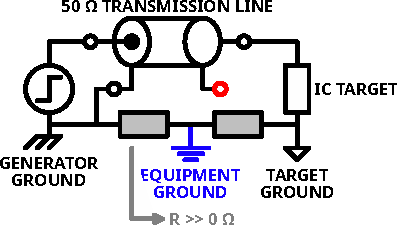
\includegraphics[width=0.5\columnwidth]{./figures/state-of-the-art-platform.pdf}}
	\subfloat[][Improved]{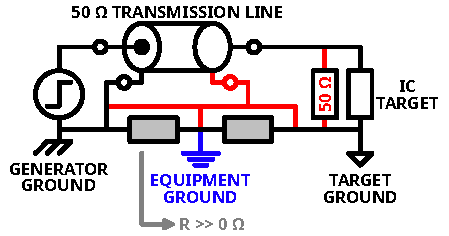
\includegraphics[width=0.5\columnwidth]{./figures/s-bbi-better.pdf}}
	\caption{Simple models of a typical (a) and an improved (b) BBI setup.}
	\label{bbi_setups}
\end{figure}

	The typical platform model is described in Fig. \ref{bbi_setups}.a and shows the main components making a BBI platform such as:
	\begin{itemize}
		\item The voltage pulse generator;
		\item The transmission line;
		\item The grounding installation;
		\item The IC target.
	\end{itemize}
	In addition to this, the schematic shows some important flaws we are going to address.
	
	While this is not always the case, voltage pulse generators are typically specified to be loaded with a 50 \textOmega\ load, or more generally with a fixed load.
	When performing BBI, the backside of the IC is electrically connected to the generator output.
	Therefore, outside of luck alone, it is very rare that the impedance presented by the IC to the generator perfectly matches the required one.
	It implies that the generator will be, most of the time, out of specifications, and that the conditions will vary depending on the chosen IC and the location of the BBI probe.
	This represents a first flaw to the typical approach.
	
	Then
	
%	Three main flaws lie in the platform in its current state:
%	\begin{itemize}
%		\item The pulse generator
%	\end{itemize}
